\section{Video Upload}
\label{sec:video_upload}
In questo paragrafo verà illustrata nel dettaglio la fase di upload dei contenuti multimediali.
La piattaforma nella parte admin permette la selezione e l'upload dei contenuti,tali operazioni sono pero incapsulate in un unico tag che innesca i processi che vedremo tra breve. 

\begin{lstlisting}[language=html]
   <form class="form">
      <input-s3-video collection="videos" folder="{{folder}}"
        response="{{video}}" error="{{error}}" on-complete="on_response">
      </input-s3-video>
    </form>
\end{lstlisting}

L'intero processo che parte con la selezione e termina con lo storage dei contenuti su AWS S3 può essere sintetizzato e chiarito con l’immagine seguente:


\begin{figure}[htb]
 \centering
 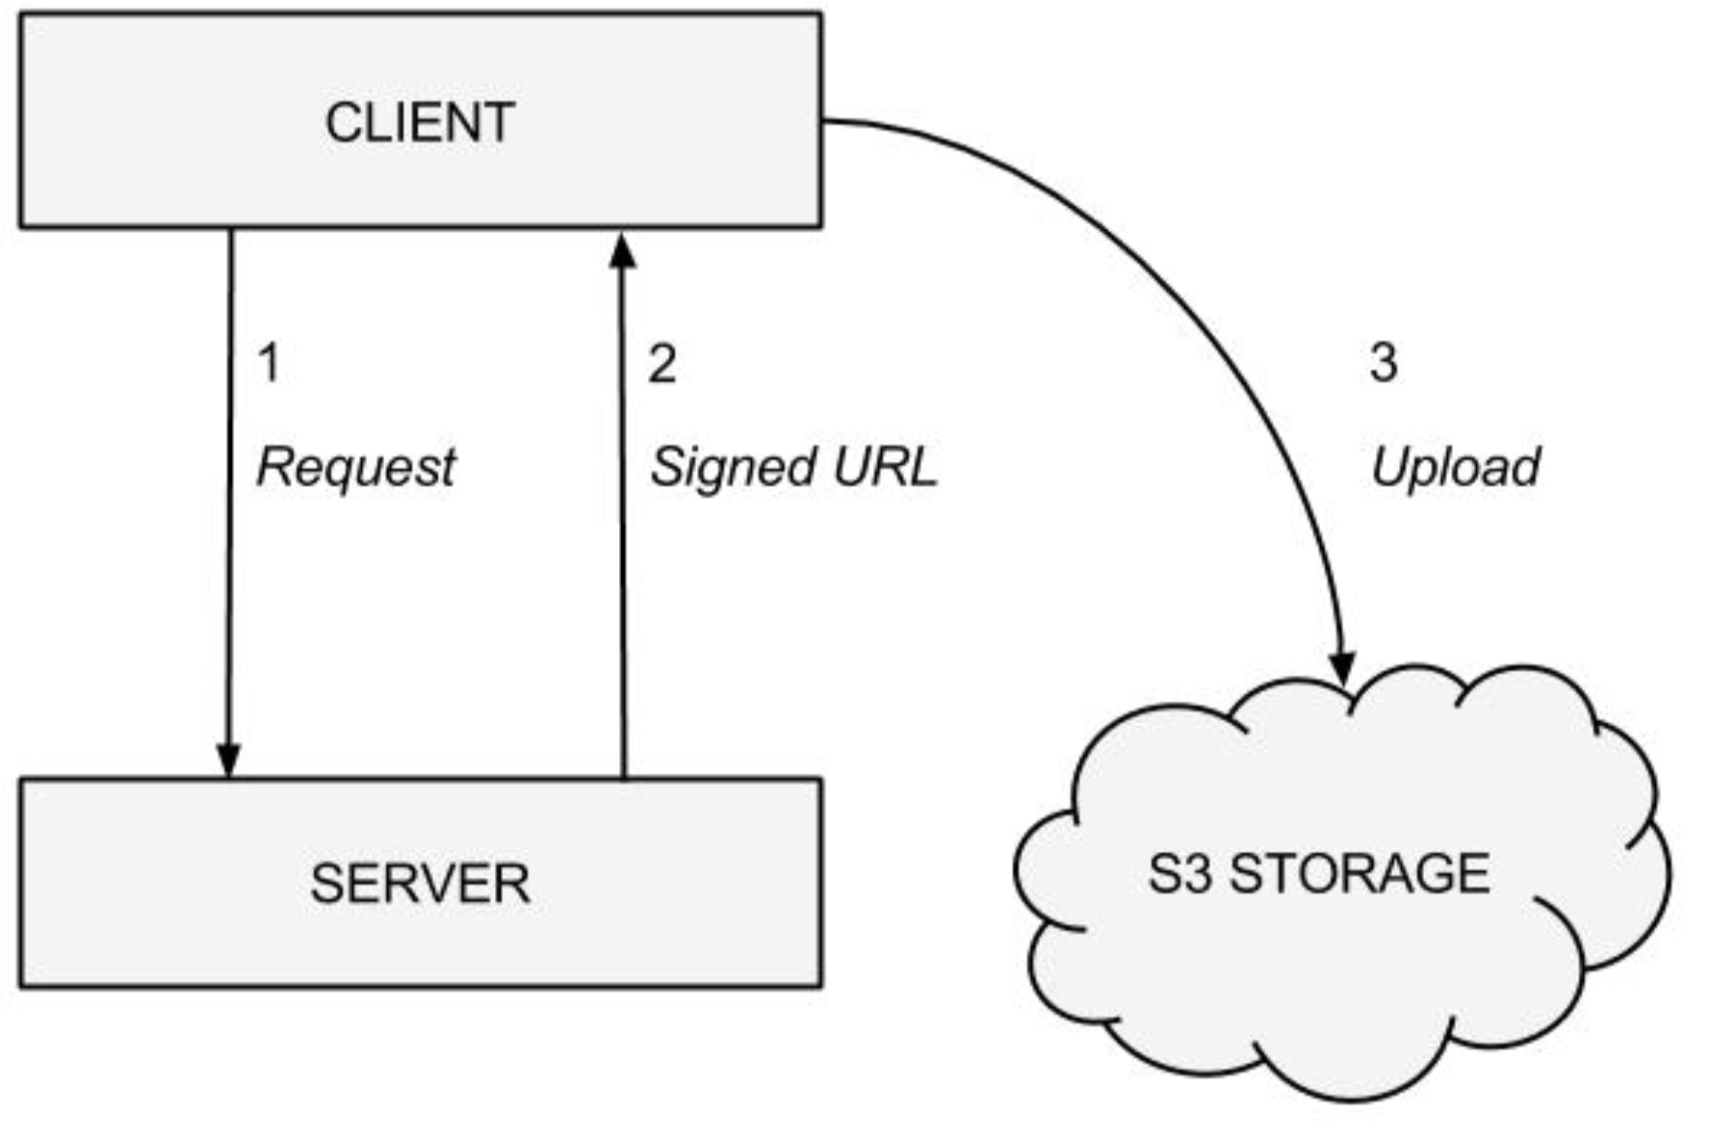
\includegraphics[width=1.0\linewidth]{images/chapter6/upload.png}\hfill
 \caption[Video upload lifecycle]{Video upload lifecycle}
 \label{fig:fourV}
\end{figure}


E’ possibile notare come il processo di upload si divide in 3 parti: 

\begin{enumerate}
\item \textbf{Request}
   Nella prima fase viene instaurata la comunicazione con Amazon AWS, quindi il client esegue una GET al server, passando:
   \begin{itemize}
      \item \textbf{params} contente il file name e file type
      \item \textbf{url} ovvero le API che devo chiamare che nel caso specifico è GET /videos/create\_multiPart\_upload
    \end{itemize}

  \begin{lstlisting}[language=html]
    <iron-ajax id="createMultiPart" method="GET" url="{{url}}" params="{{params}}"
      last-response="{{response_get}}" on-response="on_response_get">
    </iron-ajax>
\end{lstlisting}
tramite tale API viene chiamato lato server la funzione seguente che permette di stabilire la connessione con AWS e ritorna il UploadId che verrà utilizzato nei passaggi successivi per iniziare un multipart upload.

\begin{lstlisting}[language=javascript]

Video.create_multiPart_upload = function (file_name,file_type,callback){
    var s3_params = {
      Bucket: S3_BUCKET,
      Key: file_name,
      Expires: 6000,
      ContentType: file_type,
      ACL: 'public-read'      
    };
    s3.createMultipartUpload(s3_params, function(err, data) {
      if (err) {
        console.log(err, err.stack); // an error occurred
        callback(err);
        return;
      }else{
        callback(null, data);
      }
    });
  };
  
  Video.remoteMethod('create_multiPart_upload', {
    http: { verb: 'get' },
    accepts: [
      {arg: 'file_name', type: 'string'},
      {arg: 'file_type', type: 'string'}
    ],
    returns: {arg: 'UploadId', type: 'string'}
  });

\end{lstlisting}
Ottenuta la risposta da AWS, sempre lato client il contenuto multimediale selezionato per il caricamento viene suddiviso in chunks.
Il multiPart Upload può essere realizzato solo con file di dimensioni superiori a 5MB e per questo che la creazione di questi chunks viene affidata a una funzione che:
\begin{itemize}
      \item Controlla la dimensioni del file
      \item calcolo il numero di chunk in base alle dimensioni scelte per ogni chunk
      \item splitta il file in chunk, che come vedremo a breve verrano poi caricati su S3.
    \end{itemize}


\begin{figure}[htb]
 \centering
 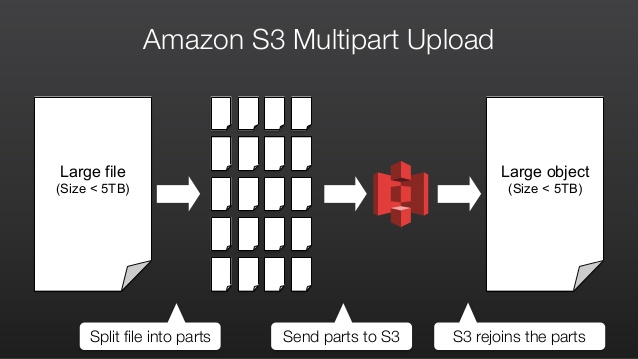
\includegraphics[width=1.0\linewidth]{images/chapter6/multipart.jpg}\hfill
 \caption[Web Components]{AWS MultipartUpload}
 \label{fig:fourV}
\end{figure}


Arrivati a questo punto iterativamente su ogni chunk viene richiesto un SignedUrl(fase 2) e poi l'upload(fae 3) su S3 come illustrato nella figura precedente:


\item \textbf{Signed URL}
  A questo punto viene di nuovo inviata una richiesta al server tramite l'API GET /videos/signed\_upload\_part.
  Tramite tale API viene chimata la funzione del server che ha il compito di chiedere ad AWS un Signed Url, e prende in input:
  \begin{itemize}
      \item Key ovvero il file name
      \item PartNumber ovvero il i-esimo chunk che sta per essere caricato
      \item UploadId ottenuto nella fase di Request

  \end{itemize}

\begin{lstlisting}[language=javascript]
  
  Video.signed_upload_part = function(Key,PartNumber,UploadId,callback) {
    var s3_params = {
      Bucket: S3_BUCKET,
      Key: Key,
      PartNumber: PartNumber, /* required */
      UploadId: UploadId /* required */
    };
    s3.getSignedUrl('uploadPart', s3_params, function (err, signed_url) {
      if (err) {
        console.log(err);
        callback(err);
        return;
      }
      callback(null, signed_url);
    });
  };

  Video.remoteMethod('signed_upload_part', {
    http: { verb: 'get' },
    accepts: [
      {arg: 'Key', type: 'string'},
      {arg: 'PartNumber', type: 'number'},
      {arg: 'UploadId', type: 'string'}
    ],
    returns: {arg: 'signed_url', type: 'string'}
  });
\end{lstlisting}

\item \textbf{Upload}

Nella terza e ultima fase si attende la risposta di AWS e quindi la Signed Url, che al suo interno conterrà l’ETAG, che rappresenta l’id dell’i-esimo chunk.
\begin{lstlisting}[language=html]
var ajax = document.createElement('iron-ajax');
        ajax.url = url;
        ajax.method = 'PUT';
        ajax.body = options.Body;
        ajax.handleAs='json';

        ajax.addEventListener('response', function (event) {
          var xhr = event.detail.xhr;
          var etag = xhr.getResponseHeader('ETag');
          var response = { etag: etag };
          resolve(response);
        });
\end{lstlisting}

come è possibile notare nello snippet sopra viene eseguita una PUT  contente le informazioni come ETAG e il chunk all’interno del body.
I punti 2 e 3 appena descritti vengono iterati per ogni chunk,e solo al termine di tutti gli upload viene comunicato a S3 il termine dell'operazione.
Quindi lato client viene viene chiamata l'API PUT /videos/complete\_upload\_part che prende in input i seguenti parametri:
  \begin{itemize}
      \item Key ovvero il file name
      \item UploadId ottenuto nella fase di Request
      \item Parts un array contente tutti gli id dei chunk

  \end{itemize}

\begin{lstlisting}[language=javascript]
Video.complete_upload_part = function(Key, UploadId,Parts,callback) {
    var s3_params = {
      Bucket: S3_BUCKET,
      Key: Key,
      UploadId: UploadId,
      MultipartUpload: {
        Parts: Parts
      } 
    };
    s3.completeMultipartUpload(s3_params, function (err, signed_url) {
      if (err) {
        console.log('ERRORE COMPLETE: ' + err);
        callback(err);
        return;
      }

      callback(null, signed_url);
    });
  };

  Video.remoteMethod('complete_upload_part', {
    http: { verb: 'put' },
    accepts: [
      {arg: 'Key', type: 'string'},
      {arg: 'UploadId', type: 'string'},
      {arg: 'Parts', type: 'array' }
    ],
    returns: {arg: 'signed_url', type: 'string'}
  });

\end{lstlisting}

\end{enumerate}
Solo al termine di tale operazione l'upload può considerarsi terminato e sarà AWS poi a ricostruire il file mettendo insieme tutti chunk ricevuti e specificati nel campo Parts della funzione precedente.
